\documentclass[12pt, a4paper, twoside, titlepage]{article}

% \usepackage{graphicx}

% \title{A not so small \LaTeX{} Article Template\thanks{To your mother}}

% \author{
% 	Your Name  \\
% 	Your Company / University  \\
% 	\and 
% 	The Other Dude \\
% 	His Company / University \\
% }

%\date{\today}

\begin{document}

(insert your text here)

% \maketitle

% \begin{abstract}
% Short introduction to subject of the paper \ldots 
% \end{abstract}

% %\tableofcontents % create a table of contens 

% \section{Introduction}
% Make it possible for all to write documents with \LaTeX{}!

% \subsection{more introduction}
% Go more in detail \ldots

% \subsubsection{even more introduction}
% come to the point \ldots

% \paragraph{Paragraphs}
% A paragraph is small but 

% \subparagraph{Subparagraphs}
% subparagraphs are smaller! 

% \paragraph{Outline}
% First we start with a little example of the article class, which is an 
% important documentclass. But there would be other documentclasses like 
% book \ref{book}, report \ref{report} and letter \ref{letter} which are 
% described in Section \ref{documentclasses}. Finally, Section 
% \ref{conclusions} gives the conclusions.



% \section{Document Classes}
% \label{documentclasses}

% \begin{itemize}
% 	\item article
% 	\item book 
% 	\item report 
% 	\item letter 
% \end{itemize}


% \begin{enumerate}
% 	\item article
% 	\item book 
% 	\item report 
% 	\item letter 
% \end{enumerate}

% \begin{description}
% 	\item[article\label{article}] {Article is \ldots}
% 	\item[book\label{book}]       {The book class \ldots}
% 	\item[report\label{report}]   {Report gives you \ldots}
% 	\item[letter\label{letter}]   {If you want to write a letter.}
% \end{description}

% \section{Tabular}
% No paper without a tabular!

% \begin{tabular}{|l|c|r|p{2cm}|}
% \hline
% first column     & second column & third column & fourth column \\
% \hline 
% l stand for left & c for center  & r for right  & and p for predefined size \\
% \hline 
% \end{tabular} 


% \section{Figure}
% No paper without a tabular!

% \begin{figure}
% 	\centering
% 	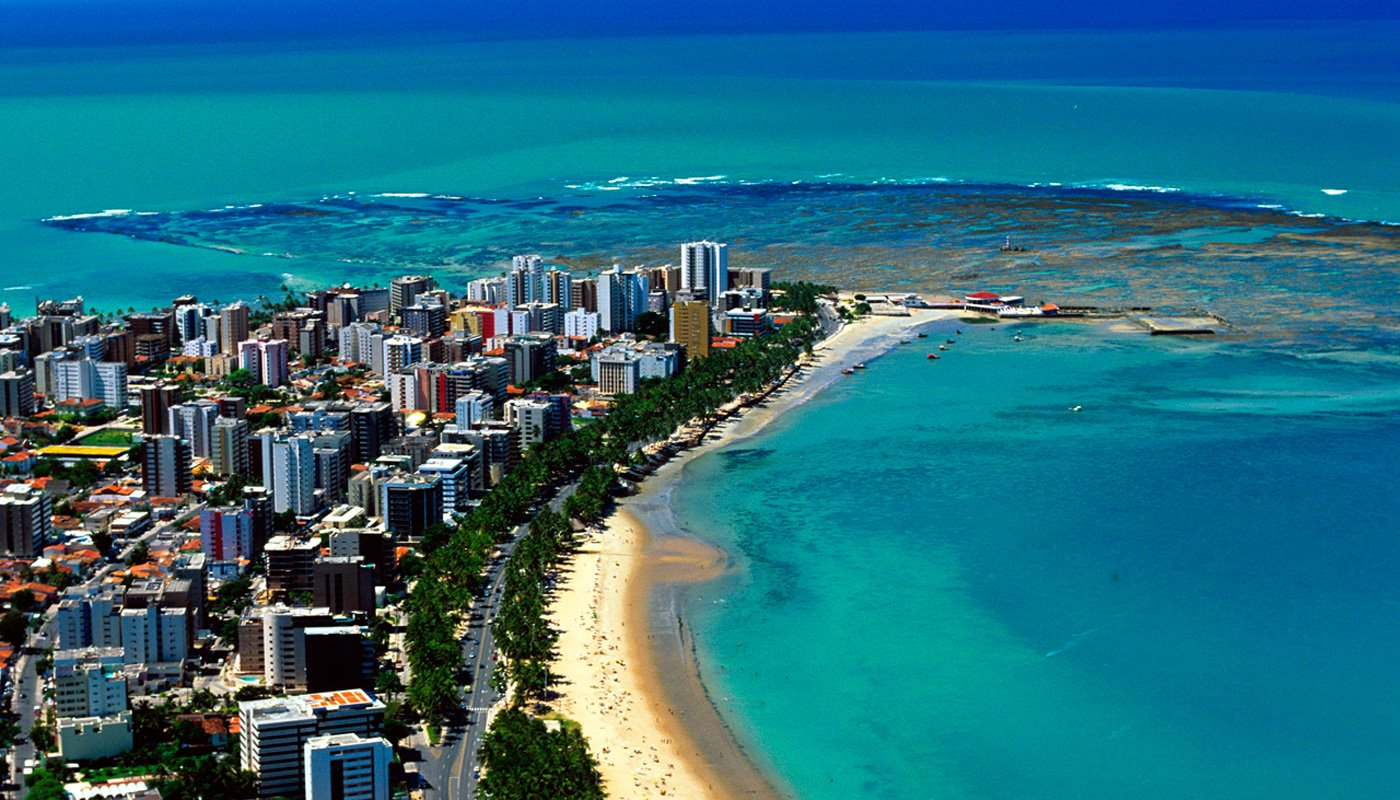
\includegraphics[width=0.5\textwidth]{maceio}
% 	\caption{Aerial view of Ponta Verde.}
% \end{figure} 


% \section{Some Math}
% Math in text is called in line math just put \$ character around 
% the math think. Like $ a^2 + b^2 = c^2 $. It looks better if you use 
% this 
% \[a^2 + b^2 = c^2\]
% or
% \begin{equation}
% a^2 + b^2 = c^2
% \end{equation}

% \section{Conclusions}
% \label{conclusions}
% There is no longer \LaTeX{} example which was written by Silveira~\textit{et al.}~\cite{Silveira2012a}.

% \bibliography{myref}
% \bibliographystyle{plain}

\end{document}